\newpage
%\pagestyle{empty}
\pagestyle{fancy}
\renewcommand{\headrulewidth}{2.4pt}
\renewcommand{\footrulewidth}{2.4pt}
\lhead{
    \setlength{\unitlength}{1mm}
    \begin{picture}(0,0)
    \put(0,0){\includegraphics[width=0.9cm]{logo.eps}}
    \end{picture}
    }
\chead{}
%\rhead{\xiaosi{合肥量子精密仪器有限公司}}
%\fancyfoot[LO,RE]{\xiaosi{ASG-GT50-C用户手册}}
\rhead{\sihao\textbf{Hefei Quantum Precision Devices Co., Ltd.}}
\fancyfoot[LO,RE]{\xiaosi{ASG-GT50-C Manual}}
\cfoot{}
\fancyfoot[RO,LE]{\xiaosi\textbf{\thepage}}



\erhao \textbf{Guaranty and Declaration}
\vspace{0.7cm}

\sihao \textbf{Trademark Information}\\
%\includegraphics[height=2cm]{logo}
%\epsfig{figure=logo,height=2cm}
%\begin{figure}[H]
%    \includegraphics[height=2cm]{logo}
%\end{figure}
\hspace*{0.8cm}\song{\qquad\qquad is a registered trademark of Hefei Quantum Precision Devices Co., Ltd.}
\hspace{-12.2cm}\includegraphics[height=2cm]{logo}

\vspace{0.8cm}
\sihao\textbf{Software Version}
\vspace{0.4cm}

\hspace{-0.2cm}We provide the sequence editing PC software in Windows and the interface program for both Windows (chapter 5) and MAC (chapter 6) system. Software upgrade might change or add product features. Please contact Hefei Quantum Precision Devices Co., Ltd. to upgrade the software. We will take the initiative to contact you if  necessary.
%\song 软件升级可能会增加或更改产品功能, 请联系合肥量子精密仪器有限公司升级软件, 必要时我司会主动与您联系。

\vspace{0.8cm}
\sihao\textbf{Notices}
%\song
\begin{itemize}
 \item Hefei Quantum Precision Devices Co., Ltd. products are covered by P.R.C. and foreign patents, issued and pending.
 \item Hefei Quantum Precision Devices Co., Ltd. reserves the right to change parts of or all the specifications and pricing policies at company's sole decision.
 \item Information in this publication replaces all previously corresponding material.
 \item Any part of this document is forbidden to be copied, photocopied, or rearranged without prior written approval of Hefei Quantum Precision Devices Co., Ltd.
 \item Once the users use the product, the whole content of this declaration shall be deemed to be recognized and accepted.
% \item 本公司产品受中国及其他国家和地区的专利( 包括已取得和正在申请的专利)保护。
% \item 本公司拥有改变产品规格及价格的权利。
% \item 本手册提供的信息取代以往出版的任何资料。
% \item 未经我司事先书面许可, 不得影印、 复制或改变本手册的任何部分。
% \item 用户一旦使用产品, 即视为对本声明的全部内容认可和接受。
\end{itemize}

\vspace{0.6cm}
%\xiaosi\textbf{产品认证}
%\vspace{3cm}

\sihao\textbf{Contact Us}
%\song
\begin{itemize}
 \item Xi Qin, CTO of Hefei Quantum Pricision Devices Co., Ltd.
 \item Email: sale@qpdtek.com
 \item Tel:  +86 13816630636
\end{itemize}

%\noindent\song
%如果您在使用此产品或本手册的过程中有任何问题或需求,可与我司联系:\\
%\song 秦熙: 合肥量子精密仪器有限公司, 首席技术官\\
%\song 电子邮箱: sale@qpdtek.com\\
% 电话: +86 13816630636

\newpage
\erhao \textbf{Safety Requirement}
\vspace{1.1cm}

\noindent\xiaosan\textbf{General Safety Summary}
\vspace{0.7cm}

\hspace{-0.4cm}To prevent potential hazards and avoid damage to the product or any device connected to this product, users need to understand the following safety measures, and use the instrument only specified by this manual.
%为避免可能的危险,以及防止损坏本产品和与本产品连接的任何设备,用户需了解以下安全措施,并按照规定使用本产品。

\vspace{0.7cm}
\noindent\sihao{\color{red}\textbf{Use Proper Power Cord}}

\vspace{0.2cm}
\hspace{-0.2cm}Only the power cord provided by our company should be used.
%只允许使用我司所提供的电源线。

\vspace{0.7cm}
\noindent{\color{red}\textbf{Power Supply should be Correct}}

\vspace{0.2cm}
\hspace{-0.2cm}To prevent damage to the product, please ensure the power supply is correct and read this manual carefully before using the product.
%为避免对操作人员造成伤害或损坏产品,请在使用产品前仔细阅读本手册,并确保产品供电电源正确。

\vspace{0.7cm}
\noindent{\color{red}\textbf{Do Not Operate Without Covers}}

\vspace{0.2cm}
\hspace{-0.2cm}Do not operate the product with covers removed.
%请勿在产品机箱打开时运行本产品。

\vspace{0.7cm}
\noindent{\color{red}\textbf{Avoid exposure of Circuit}}

\vspace{0.2cm}
\hspace{-0.2cm}Do not touch exposed junctions and components when the unit is powered, and please contact with us immediately.
%若机箱内电路板元件有外露, 请勿触碰并立即与我司联系。

\vspace{0.7cm}
\noindent{\color{red}\textbf{Keep Well Ventilation}}

\vspace{0.2cm}
\hspace{-0.2cm}To prevent the increase of instrument temperature which would cause damage to the product, please keep the instrument well ventilated and do not block the air vents.
%为避免因机箱内电路板过热而损坏仪器,在使用本产品的过程中请勿堵住通风口。

\vspace{0.7cm}
\noindent{\color{red}\textbf{Do Not Operate in Wet Conditions}}

\vspace{0.2cm}
\hspace{-0.2cm}In order to avoid short circuiting to the interior of the device or electric shock, please do not operate the instrument in a humid environment.
%为避免产品内部电路出现短路等危险情况, 请勿在潮湿环境下操作仪器。


\vspace{0.7cm}
\noindent{\color{red}\textbf{Do Not Operate in an Explosive Atmosphere}}

\vspace{0.2cm}
\hspace{-0.2cm}In order to avoid personal injuries or damage to the device, it is important to operate the device away from an explosive atmosphere.
%为避免人身伤害或产品损坏, 严禁易燃易爆物靠近本产品。

\vspace{0.7cm}
\noindent{\color{red}\textbf{Handling Safety}}

\vspace{0.2cm}
\hspace{-0.2cm}Please handle carefully during transportation to avoid damage to keys, interfaces, LED and other parts on the panels.
%为避免对产品面板上的按键、 接口、 指示灯等部件造成损坏, 请注意搬运安全。

\vspace{0.7cm}
\noindent{\color{red}\textbf{Do Not Place the Product in High Temperature Environment}}

\vspace{0.2cm}
\hspace{-0.2cm}To prevent potential hazards, it is forbidden to place the product in high temperature environment.
%为避免发生危险,严禁将本产品放置于高温环境中。

%\newpage
\vspace{0.7cm}
\noindent{\color{red}\textbf{People Who do not Have Ability are Forbidden to Operate the Product}}

\vspace{0.2cm}
\hspace{-0.2cm}In order to avoid personal injuries or damage to the device, people who do not have operation ability such as the olds and kids, are forbidden to use the product.
%为避免造成人身伤害或产品损坏,严禁不具备操作能力的人( 如老人、 儿童)使用本产品。

\vspace{0.7cm}
\noindent{\color{red}\textbf{General Care and Cleaning}}

\vspace{0.2cm}
\hspace{-0.2cm}Please clean the instrument regularly. To clean the exterior surface, perform the following steps: disconnect the instrument from all power sources, then clean the dust on the panel of the instrument with a dry cloth.
%请经常对产品进行清洁, 方法如下: 先断开电源, 再用干抹布轻轻擦拭产品机箱外部。

%\vspace{0.6cm}
%\noindent{\color{red}\textbf{怀疑产品出故障时, 请立即联系我司}}
%
%如果您怀疑本产品出现故障, 请联络我司授权的维修人员进行检测。 任何由未经我司允许的维护、 调整或零件更换而造成损失, 我司不承担任何责任。

\newpage
%\pagestyle{plain}
%\setcounter{page}{1}
\noindent\huge \textbf{ASG-GT50-C Series Overview}
\vspace{0.6cm}

\normalsize ASG-GT50-C serials are high performance pulse/delay generators named Arbitrary Sequence Generators. The device provides 8 independent pulse output channels. As shown in Fig 1, the width of each positive pulse could be adjusted from 7.5 ns to 2.6 s, and negative pulse could be adjusted from 10.0 ns to 2.6 s, which is no dead time with 50 ps time resolution.
\begin{figure}[ht]
\centering
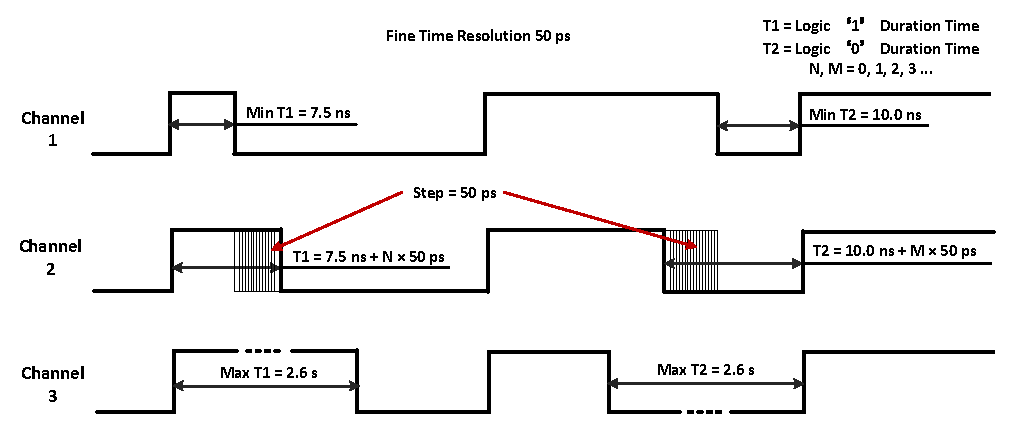
\includegraphics[width=14.5cm,height=6cm]{fig_shixu}
\caption{\hspace{0.2cm}Time diagram of pulse signals}\label{fig:fig1}
\end{figure}
\vspace{0.5cm}

\makeatletter
\def\hlinewd#1{%
  \noalign{\ifnum0=`}\fi\hrule \@height #1 \futurelet
   \reserved@a\@xhline}
\makeatother
%\newcommand\vlinewd#1{\vrule width #1}
\definecolor{myblue}{rgb}{.46,.42,.80}
\definecolor{tabcolor_top}{rgb}{255,255,255}
\definecolor{tabcolor}{rgb}{255,255,255}
\noindent\sanhao\textbf{Main Features}
%\vspace{0.1cm}
\song
\begin{table}[H]
\normalsize
\rowcolors{2}{gray!20}{gray!20}
\begin{tabular}{m{13.5cm}}
\rowcolor{gray!20}
\arrayrulecolor{tabcolor_top}\toprule[1.8pt]
Time Resolution: 50 ps\\\arrayrulecolor{tabcolor}\midrule[1.2pt]
Maximum Number of Channels: 8 \\\arrayrulecolor{tabcolor}\midrule[1.2pt]
Dynamic Range of  Single Pulse Width: from 7.5 ns  to  2.6 s\\\arrayrulecolor{tabcolor}\midrule[1.2pt]
Long-term jitter: < 25 ps (Pulse width = 500 ms) \\\arrayrulecolor{tabcolor}\midrule[1.2pt]
Sequence storage memory: 4 GB\\\arrayrulecolor{tabcolor}\midrule[1.2pt]
USB Interface\\\arrayrulecolor{tabcolor}\midrule[1.2pt]
Provide sequence editing PC software\\
\arrayrulecolor{tabcolor_top}\bottomrule[1.8pt]
\end{tabular}
\end{table}

%\begin{itemize}
% \item 50 ps时间分辨率的方波输出。
% \item 8个通道独立自定义方波输出。
% \item 单脉冲动态范围为5 ns至2.6 s,且无死时间。
% \item 高长期稳定度。
% \item 集成了高速计数读出功能。
% \item 方波序列的存储内存可以达到4 GB。
% \item 采用USB接口通信。
% \item 配备方波序列编辑软件。
%\end{itemize}

%\vspace{0.5cm}
%\newpage
\vspace{0.2cm}
%\noindent\xiaosan\textbf{Performance Characteristics}
\noindent\xiaosan\textbf{Product Specifications}
\vspace{0.5cm}

\noindent\sihao\textbf{Appearance Characteristics:}
\vspace{0.1cm}
\song
\begin{table}[H]
\normalsize
\rowcolors{2}{gray!20}{gray!20}
\begin{tabular}{m{6.5cm}|m{6.5cm}}
\rowcolor{myblue}
%\arrayrulecolor{tabcolor_top}\toprule[1.8pt]
\color{white}Parameter& \color{white}Value\\\arrayrulecolor{tabcolor}\midrule[1.2pt]
Material of the Case& Aluminium alloy\\\arrayrulecolor{tabcolor}\midrule[1.2pt]
Color& Silver gray\\\arrayrulecolor{tabcolor}\midrule[1.2pt]
Size& 207*122*65 mm\\
%\arrayrulecolor{tabcolor_top}\bottomrule[1.8pt]
\end{tabular}
\end{table}

%\begin{itemize}
 %\item 机身材质: 铝合金外壳
 %\item 机身颜色: 银灰色
 %\item 产品尺寸: 207*122*65 mm
%\end{itemize}

\vspace{0.4cm}
%\newpage
\noindent\sihao\textbf{Electrical Characteristics:}
\vspace{0.1cm}
\song
\begin{table}[H]
\normalsize
\rowcolors{2}{gray!20}{gray!20}
\begin{tabular}{m{6.5cm}|m{6.5cm}}
\rowcolor{myblue}
%\arrayrulecolor{tabcolor_top}\toprule[1.8pt]
\color{white}Parameter& \color{white}Value\\\arrayrulecolor{tabcolor}\midrule[1.2pt]
Operating Voltage& DC 12 V\\\arrayrulecolor{tabcolor}\midrule[1.2pt]
Standby Current& About 0.85 A\\\arrayrulecolor{tabcolor}\midrule[1.2pt]
Operating Current& ≤ 1.2 A\\\arrayrulecolor{tabcolor}\midrule[1.2pt]
Maximum Power& About 12 W\\
%\arrayrulecolor{tabcolor_top}\bottomrule[1.8pt]
\end{tabular}
\end{table}

%\begin{itemize}
% \item 工作电压: DC 12 V
% \item 待机电流: 约 0.85 A
%\item 工作电流: ≤1.2 A
 %\item 最大功率: 约 12 W
%\end{itemize}

\vspace{0.4cm}
\noindent\xiaosi\textbf{Technical Parameters:}
\vspace{0.1cm}
%\song
\begin{table}[H]
%\Large
\rowcolors{2}{gray!20}{gray!20}
\begin{tabular}{m{6.5cm}|m{6.5cm}}
\rowcolor{myblue}
%\arrayrulecolor{tabcolor_top}\toprule[1.8pt]
\color{white}Parameter& \color{white}Value\\\arrayrulecolor{tabcolor}\midrule[1.2pt]
Time Resolution& 50 ps\\\arrayrulecolor{tabcolor}\midrule[1.2pt]
Minimum pulse width& 7.5 ns \\\arrayrulecolor{tabcolor}\midrule[1.2pt]
Maximum pulse width& 2.6 s\\\arrayrulecolor{tabcolor}\midrule[1.2pt]
Maximum Number of Channels& 8\\\arrayrulecolor{tabcolor}\midrule[1.2pt]
Sequence storage memory& 4 GB\\\arrayrulecolor{tabcolor}\midrule[1.2pt]
Maximum Number of Pulses ( single channel )&  4×$10^{7}$\\\midrule[1.2pt]
Coupling& DC 50 ohm\\\arrayrulecolor{tabcolor}\midrule[1.2pt]
Output Low Voltage& 0 V\\\arrayrulecolor{tabcolor}\midrule[1.2pt]
Output High Voltage& 3.3 V\\\arrayrulecolor{tabcolor}\midrule[1.2pt]
%\arrayrulecolor{tabcolor_top}\bottomrule[1.8pt]
\end{tabular}
\end{table}


%\begin{itemize}
% \item  时间分辨率: 50 ps
% \item 最小脉冲宽度: 5 ns
% \item 最大脉冲宽度: 2.6 s
% \item 最大方波输出通道数: 8
% \item  方波序列存储内存: 4 GB
%\item  单通道最多输出方波个数: $4\times 10^8$个
% \item  耦合方式: DC 50 ohm
% \item  输出低电平: 0 V
% \item  输出高电平: 3.3 V
% \item  输入低电平: -5.2 V 至 +0.4 V
% \item  输入高电平: +0.6 V 至 +3.5 V
% \item  最大计数率: 50 MHz
% \item  单个计数使能信号脉冲宽度范围: 5 ns 至 5000 s
%\end{itemize}

\vspace{0.4cm}
%\newpage
\noindent\sanhao\textbf{Applications:}
\vspace{0.3cm}
\song
\begin{table}[H]
%\Large
\rowcolors{2}{gray!20}{gray!20}
\begin{tabular}{m{13.5cm}}
\rowcolor{gray!20}
\arrayrulecolor{tabcolor_top}\toprule[1.8pt]
High resolution pulse/sequence generations\\\arrayrulecolor{tabcolor}\midrule[1.2pt]
High precision synchronization \\\arrayrulecolor{tabcolor}\midrule[1.2pt]
Delay Generations\\\arrayrulecolor{tabcolor}\midrule[1.2pt]
\arrayrulecolor{tabcolor_top}\bottomrule[1.8pt]
\end{tabular}
\end{table}

\newpage
\qquad

%\begin{itemize}
 %\item 高时间精度的脉冲/序列发生器
 %\item 延时发生器
 %\item 高精度计时器
 %\item 高精度同步器
 %\item 高速计数读出
%\end{itemize}
